\documentclass[12pt,a4paper]{scrartcl}
\usepackage{amsmath}
\usepackage{mathtools}
\usepackage{graphicx}
\usepackage[english]{babel}
\usepackage{float}
\usepackage{multirow}
\usepackage[T1]{fontenc}
\usepackage{lmodern}
\usepackage[export]{adjustbox}
\setlength{\parskip}{6pt}
\setlength{\parindent}{0pt}

\graphicspath{pics/}

\begin{document}
\title{Development and Programming of a Micro Processor}
\author{Alisa Dammer and Sven-Hendrik Haase}
\maketitle

\tableofcontents

\newpage

\section{Introduction}
\subsection{General Information: How a CPU works}
A Central Processing Unit (CPU) is the heart of a computer. It performs arithmetic operations, logic operations and input/output operations. Nowadays computers generally have very complex and smart CPUs which can perform many billions of operations in a second. However, in our project we have concentrated our attention on developing a rather simple micro processor and its supporting tools.

In order to work properly and execute commands (perform certain operations), a CPU needs to go through several stages:
\begin{enumerate}
	\item Fetch: Read a program that is stored in memory as a list of instructions. We implemented an assambler that translates the program from a human-readable language to machine code. More about it in the section "CPU implementation". To keep an eye on the correct order of the instructions, the program Counter (PC) keeps track of the address of the next executable instruction in ROM.
	\item Decode: An instruction is a representation of an assembly command in one or more bitstrings. During this stage every instruction is broken up into several parts. The amount and length of these pieces depend on the type of instruction (more details in the next section). 
	\item Execute: According to what kind of instruction has to be performed, different units of the CPU can be involved. For example: an ALU and two registers, or a CU and a register bank etc. Normally modern CPUs have overflow flags, that are "activated" if the output is larger than the register can deal with.
	\item Return: During this stage the result of an instruction is returned to a register so that it could be used later on.
\end{enumerate}

For every instruction in a program all four phases are executed. The cycle works until the \texttt{stop} instruction is reached, which is normally refered to a \textbf{program termination}. As was mentioned above in the Fetch-stage, the program counter holds the address of the next executable instruction, incrementing each time the instruction is executed. Some of the control instructions like \texttt{jump} change the PC according to the needs of the program, for example by implementing a loop.

\subsection{Main Components of a Simple CPU}
Every CPU's design starts with an Instruction Set Architecture (ISA) definition that describes what a particular processor is capable of: general specification (word length, instruction length), instruction specifications and opcodes (operations that are presented in binary form), types of memory that are used (ROM, RAM, special) as well as number of special purpose and general purpose registers, and other specific information if needed.

In order to make the processor perform things listed in ISA all micro processors have certain units like: Program Counter (PC), Control Unit (CU), Arithmetic Logic Unit (ALU), Registers (Register Bank), Buses.\\

\begin{figure}[h]
	\centering
	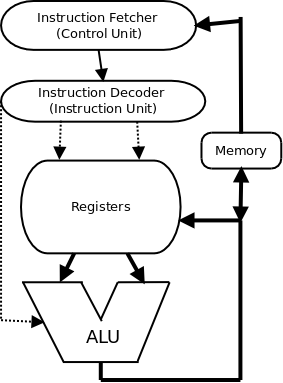
\includegraphics[scale=0.6]{pics/simpleCPU3.png}
	\caption{General microprocessor model}
\end{figure}

\newpage
\section{CPU implementation}
\subsection{Instruction Set Architecture}
As was mentioned in the previous section, ISA defines all specifications of a CPU. In this project we decided to use 16-bit instructions that have the same length as a word, so that we didn't have to think about instructions consisting of more than one word and thus we didn't need to deal with proper splitting of the instruction  which also makes the Instruction Unit (our instruction decoder) easier to implement.
\begin{verbatim}
general specifications:
    16 bit instructions
    16 bit words
    14 registers:
        8 general purpose registers
        6 special purpose registers
\end{verbatim}

The CPU in our implementation uses only one type of instruction. We don't have special flags. Instead of special flags, we use special purpose registers and certain instructions. As was already mentioned: we have implemented a pretty simple micro processor.
\begin{figure}[h!]
	\centering
	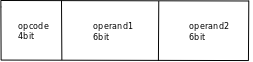
\includegraphics[scale=0.6]{pics/instruction1.png}\\
	\caption{Instruction type}
\end{figure}
Because we have set the length of opcode to 4 bits, we could have a maximum of 16 (\(2^4\)) opcodes only. We managed to expand this pool of opcodes with a set of pseudo instruction that the compiler will expand to opcode-based instructions. They are replaced with a composition of actual instructions (sequence of actual instructions that leads to the same result). For example, an instruction "add" operates with two registers, saving result of the operation to the left (or to the first) register:
\begin{verbatim}
movi a 5
movi b 4
add a b
stop
\end{verbatim}
This program will result in:
\begin{verbatim}
program start
PC0 => movi a 7
PC1 => movi b 4
PC2 => add a b
program end
\end{verbatim}
The result register \texttt{a} gets the value \(11 = 7 + 4\). We didn't implement any special output register because we can always store (or move to desirable output register) data manually to certain location in the memory, that we agreed will hold the final result.\\
A complete list of all instructions can be found in the Appendix.

As previously stated, pseudo instructions can be represented by a composition of actual instructions. Some of them consist of two instructions, some of them contain up to five instructions. For example:
\begin{verbatim}
movi a 7
addi a 5
stop
\end{verbatim}
The original program consists of three instructions, but it results in program with four instructions, because \texttt{addi} is a pseudo instruction and it consists of a composition of \texttt{movi} and \texttt{add} instructions.
\begin{verbatim}
program start
PC0 => movi a 7
PC1 => movi tmp1 5
PC2 => add a tmp1
program end
--------------------
\end{verbatim}
Another example for a pseudo instruction is a program that implements modulo, calculating \(45 \mod 10 \equiv 5\)
\begin{verbatim}
movi a 45
movi b 9
mod a b
stop
\end{verbatim}
It will result in:
\begin{verbatim}
program start
PC0 => movi a 45
PC1 => movi b 10
PC2 => mov tmp1 a
PC3 => div a b
PC4 => mul a b
PC5 => sub tmp1 a
PC6 => mov a tmp1
program end
--------------------
registers:
pc: 7
tmp1: 5
a: 5
b: 10
\end{verbatim}
Apart from instructions (opcodes) and general information, ISA gives information about registers: general and special purpose.
\newpage
\begin{verbatim}
registers:
    zero 		000000 # always returns value 0
    pc			000001 # program counter
    cmp_result  000010 # result of comparison as defined below
    jmp_next    000011 # je will go here if the comparison succeeds
    tmp1        000100 # temporary register to be used by compiler
    tmp2		000101 # another temporary register

    # general purpose registers
    a           000110
    b           000111
    c      	    001000
    d           001001
    e           001010
    f           001011
    g           001100
    h           001101
\end{verbatim}

In our project we have decided not to implement ALU and Control Unit separately as MyHDL conveniently allows us to structure our project differently (actually, at the beginning we tried to implement all units separately and then unite them inside of the Control Unit, but we have run into difficulties).\\

The complete pipeline for running a program written in our assembly has the following stages:
\begin{enumerate}
	\item Encode - Assembly programm is translated with the help of the Assembler. The output file is an object file that the CPU can directly load and execute. The output file consists of N 16-bit bitstrings, where N is the number of actual instructions (here, if a pseudo instruction is used in the program, it is translated into several actual instructions for further executing). So, as the result we get machine code.
	\item Program Loading - The program needs to be loaded into ROM in order to be accessible to the CPU. In our case, the simulation takes care of that and puts the instructions into the ROM as a list of 16-bit integers.
	\item Decode - The current instructed pointed at by the PC is loaded into the Instruction Unit which splits it into three parts: opcode, operand1 and operand2. As the result of this stage we get executable instructions, where the Control Unit knows what operations with which operands is to be performed. 
	\item Execution - At this point the Control Unit actually runs the operations with the given values, using both memory and registers accordingly. As the result of the executing of a program we get the result as a change of CPU state in either RAM or registers.\\
	
Our CPU can be presented as the following schema:
\end{enumerate} 

\begin{figure}[h]
	\centering
	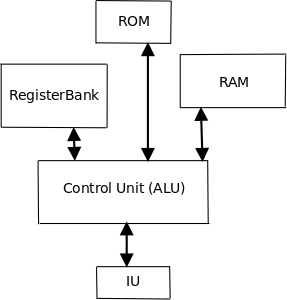
\includegraphics[scale=0.6]{pics/ourCPU.png}\\
	\caption{Our CPU schema}
\end{figure}

\newpage
\subsection{Assembler}
As mentioned above, our first stage of the program execution is the encoding of the program. This happens in assempler.py unit in following order:
\begin{enumerate}
	\item An input assembly file is opened.
	\item Every input line of the file is translated to its corresponding instruction bitstring.
	\item Depending on type of instruction, whether it is an actual or pseudo instruction, the command will be converted into one or more opcode-based instructions. Every bitstring is appended to the binary file.
\end{enumerate}
The bitstring output list for our modulus program above, for example, looks like this:
\begin{verbatim}
alisa@comrade ~/u/proj> python2 assembler.py programs/test.asm
['0100000110101101', '0100000111001001', '0011000100000110',
 '1000000110000111', '0111000110000111', '0110000100000110',
 '0011000110000100', '0000000000000000']
\end{verbatim} 
Our assembler is a simple parser supporting labels. It contains a state machine for all instructions mentioned in the ISA so that the Control Unit (in our case also ALU) deals only with actual opcodes as it can't directly execute pseudo instructions.\\

\subsection{Memory and Registers}
Every processor has a memory unit - a physical subdevice to allow for storing the program in reprogrammable memory and to allow for programs to access vast amounts of dynamic data. We disambiguate between two primary types of memory: non-volatile (flash memory,  ROM/PROM/EPROM/EEPROM) and volatile (RAM, DRAM).

Non-volatile memory is normally used for storing information for long-term use without its change. However, current non-volatile memory implements are rather slow for their immediate use in a processor and thus not efficient for temporary and local computations).

In our implementation, our simulation loads the program before the CPU is initialized and then "burns" the ROM into the CPU. Our ROM has three parameters: Rom(dout, addr, CONTENT). The first two are the output value and memory location respectively. The third parameter is initialized with the help of a special function "load\_program(path)" that is implemented in the simulation loader.

Currently the most commonly used types of a volatile memory (RAM) are static RAM (SRAM) and dynamic RAM (DRAM). Since we have a simulation only, we didn't have to work with a specific memory type. It should be noted, however, that we set up our RAM in such a way that MyHDL should be able to generate code that uses an FPGA's hardware RAM if it has one.

In this project RAM is limited with to 32 memory cells that can store a word each. As such, both RAM and ROM can hold value up to $2^{16}$.

We can simultanously operate on a register, RAM and ROM at the same time as they all have different buses. Perhaps the only mistake we made in the implementation of the memory system is that we can only communicate with the registers using a single channel as opposed to having one channel per register. This effectively makes registers just as inefficient as using RAM directly.

Apart from the (non-)volatile memory we have implemented a register bank that consists of 14 registers split into two groups: general purpose and special purpose registers.

Since our CPU is quite limited, we don't need many registers to work with. We have implemented several special purpose registers to partially substitute flags and some hardware units. For example we have a pc register that gets/holds the address of the next instruction directly from the CU (we don't have a self-sufficient Program Counter. In our case the number of the next instruction is the number of the line where a particular instruction is located).

\subsection{Instruction Unit}
Since we have restricted the length of words and instruction size to the same value (16-bit, or 2-byte), decoding an instruction became really easy:
According to the ISA, an instructions look like this:
\begin{verbatim}
	[4-bit opcode][6-bit operand1][6-bit operand2]
\end{verbatim} 
In the case of opcodes that don't need operands or only need a singe operand, the other bits are ignored.

For example:

\begin{verbatim}
movi a 3
movi b 9
not a b
stop
\end{verbatim}
Will result in:
\begin{verbatim}
program start
PC0 => movi a 45
PC1 => movi b 9
PC2 => not a
program end
--------------------
registers:
zero: 0
pc: 3
cmp_result: 0
jmp_next: 0
tmp1: 0
tmp2: 0
a: 65533
b: 9
\end{verbatim}
As you can see, the second operand influences neither the execution of the program, nor the correctness of the result.

\subsection{Control Unit}
Classically, the Control Unit (CU) handles the operation of the whole processor, it manages communication between input and output devices, interpretes and executes them itself (in our case), or via delegation of some operations to the ALU. Also, the Control Unit provides control signals, like clock (clk in our code). The CU performs all four stages of a program execution.\\
In our project the Control Unit is implemented inside of the simulation module. Register Bank and Instruction Unit are controlled by the CU but as separate units (instances are initialized before the implementation of the Control Unit itself). The Program Counter, usually, is a self-sufficient unit that is implemented outside the CU but in our case is also built-in into the Control Unit. Since we have a special register for the address of the next instruction (\texttt{pc} register), the CU has two ways of changing the \texttt{pc} register. These two ways are:
\begin{enumerate}
	\item The instruction is already executed, and certain operations are successfully performed. Afterwards the value in the \texttt{pc} register is  incremented (in the \textbf{Memory and Registers} section it was shown how the PC tracks the executable instruction). 
	\item The second possibility to change the PC is using flow control instructions (Jump instructions, see Appendix). These are jump opcodes. Here in the special purpose register "jmp\_next" the location of the jump (the address of the next desirable instruction) is stored. If the condition of the jump operation matches the result, the PC gets set to the value from jmp\_next-register.
\end{enumerate}

\newpage
\section{Results}
\subsection{Test of the CPU}
Now, in order to demonstrate our CPU, we'll present a more complicated test to show it off: The Euclidean algorithm for calculating the greatest common divisor.

The way this algorithm works is:
\begin{verbatim}
function gcd(a, b)
    while b != 0
       t := b
       b := a mod b
       a := t
    return a
\end{verbatim}

First we need to write the program in assembly:

\begin{verbatim}
0.  movi a 45
1.  movi e 3
2.  movi f 2
3.  movi b 3
4.  shift_l a e
5.  shift_l b f
6.  mov g a
7.  mov h b
8.  movi c 0
9.  .loop
10. movi jmp_next .loop
11. mov d b
12. mod a b
13. mov b a
14. mov a d
15. jne b c
16. stop
\end{verbatim}
The assembly encoding of the program looks like:
\begin{verbatim}
alisa@comrade ~/u/proj> python2 assembler.py programs/ggt.asm
['0100000110101101', '0100001010000011', '0100001011000010',
 '0100000111000011', '1100000110001010', '1100000111001011',
 '0011001100000110', '0011001101000111', '0100001000000000',
 '0100000011001001', '0011001001000111', '0011000100000110',
 '1000000110000111', '0111000110000111', '0110000100000110',
 '0011000110000100', '0011000111000110', '0011000110001001',
 '1110000111001000', '0100000100000001', '1111000100000010',
 '0100000100000010', '1111000100000010', '0000000000000000']
\end{verbatim}
The binary file has 24 instructions because of the several pseudo instructions in the original program. Since the Control Unit in our project deals only with the opcodes of the actual operations the assembler writes back the composition of actual instructions for each pseudo instruction used in the code.\\
The next step is simulation of the program, using the output file "ggt.o"
\begin{verbatim}
alisa@comrade ~/u/proj> python2 simulation.py programs/ggt.o
program start
PC0 => movi a 45
PC1 => movi e 3
PC2 => movi f 2
PC3 => movi b 3
PC4 => shift_l a e
PC5 => shift_l b f
PC6 => mov g a
PC7 => mov h b
PC8 => movi c 0
PC9 => movi jmp_next 9
PC10 => mov d b
PC11 => mov tmp1 a
PC12 => div a b
PC13 => mul a b
PC14 => sub tmp1 a
PC15 => mov a tmp1
PC16 => mov b a
PC17 => mov a d
PC18 => cmp b c
PC19 => movi tmp1 1
PC20 => je tmp1 cmp_result
PC21 => movi tmp1 2
PC22 => je tmp1 cmp_result
program end
--------------------
registers:
zero: 0
pc: 23
cmp_result: 0
jmp_next: 9
tmp1: 2
tmp2: 0
a: 12
b: 0
c: 0
d: 12
e: 3
f: 2
g: 360
h: 12
memory:
0: 0    1: 0    2: 0    3: 0
4: 0    5: 0    6: 0    7: 0
8: 0    9: 0    10: 0   11: 0
12: 0   13: 0   14: 0   15: 0
16: 0   17: 0   18: 0   19: 0
20: 0   21: 0   22: 0   23: 0
24: 0   25: 0   26: 0   27: 0
28: 0   29: 0   30: 0   31: 0
\end{verbatim}

The result of the program is stored register a. It has value = 12, that is indeed the GCD of 360 (shift\_l 45 3) and 12 (shift\_l 3 2).\\
In this program we havn't used RAM (but we could potentialy run the computation through the memory or keep some result there).
Also, in order to see the clock synchronization, you can look on the wave diagram of the project:

\begin{figure}[h]
	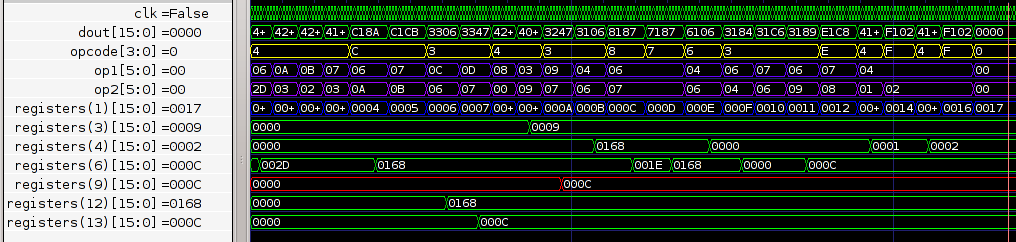
\includegraphics[scale=0.7,center]{pics/gtkwave.png}
	\caption{General microprocessor schema}
\end{figure}

\newpage
\subsection{Post Mortem}
During the realization of the project we have used MyHDL, which is a Python library for HDL. It enables VHDL and Verilog output.

We also ran into a bunch of issues that working in a highly parallel environment comes with.
The first difficulty was the synchronizing. In the beginning we decided to implement "classical" circuit - all units had to be implemented seperatly (distinct unit on a circuit), which was a problem without a central place to clock and synchronize all the units.

The obvious limitation for word and instruction size didn't give us a lot of room for opcodes. As a result, we had to resort to adding lots of pseudo instructions which in turn results in more code being generated and thus increasing the time the program needs to be completely executed. 

\newpage
\section{Appendix}
\subsection{ISA}
\begin{tabular}{|c|c|c|c|}
\hline
Class & Operation & Example & Binary Example\\
\hline
\multirow{11}{*}{Arithmetic} & add & add a b & 0101 000110 000111 \\
& addi & addi a 3 & pseudo \\
& sub & sub a b & 0110 000110 0000111\\
& subi & subi a 6 & pseudo\\
& mul & mul a b & 0111 000110 0000111\\
& muli & muli a 2 & pseudo\\
& div & div a b & 1000 000110 0000111\\
& divi & divi a 3 & pseudo\\
& inc & inc a b & pseudo\\
& dec & dec a 3 & pseudo\\
& swap & swap a b & pseudo\\
\hline
\multirow{6}{*}{Logical} & not & not a & 1001 000110 000000\\
& and & and a b & 1010 000110 000111\\
& or & or a b & 1011 000110 000000\\
& xor & xor a b & pseudo\\
& nand & nand a b & pseudo\\
& nor & nor a b & pseudo\\
\hline
\multirow{2}{*}{Shift} & shifl\_l & shift\_l a b & 1100 000110 000111\\
& shifl\_r & shift\_r a b & 1101 000110 000111\\
\hline
\multirow{7}{*}{Jump} & j & j & pseudo \\
& je & je a b & 1111 000110 000111 \\
& jne & jne a b & pseudo \\
& jg & jg a b & pseudo \\
& jge & jge a b & pseudo \\
& jl & jl a b & pseudo \\
& jle & jle a b & pseudo \\
\hline
\multirow{4}{*}{Memory} & store & store a b & 0001 000110 000111\\
& load & load a b & 0010 000110 000111\\
& mov & mov a b & 0011 000110 000111\\
& movi & movi a 5 & 0001 000110 000101\\
\hline
\multirow{2}{*}{Flow} & stop & stop & 0000 000000 000000 \\
& noop & noop & pseudo \\
\hline
\end{tabular}
\end{document}

